%!TEX program = xelatex
\documentclass[a4paper]{ctexart}

\usepackage{listings} 
\usepackage{geometry}
\usepackage{booktabs}
\usepackage{graphicx}
\usepackage{tabularx}
\usepackage{multirow}
\usepackage{enumitem}
\usepackage[bottom]{footmisc}

\renewcommand{\multirowsetup}{\centering}

\geometry{
    left=23mm,
    right=23mm,
    top=23mm,
    bottom=23mm,
}

\setlength{\parskip}{0.5em}

\title{\Huge PetLover 项目启动文档}

\author{
  陈梓俊 191250016\\
  丁炳智 191250024\\
  姬筠刚 191250055\\
  刘庭烽 191250093\\
}
\date{\today}

\begin{document}

\maketitle

\centerline{
\includegraphics[]{logo.png}}

\newpage

\begin{abstract}
  此处添加摘要
\end{abstract}



\tableofcontents

\newpage

\setlength{\parskip}{1em}


\section{项目简介}



\section{度量数值}

添加度量数值

\section{商业模式画布}

\subsection{要点概述}

商业模式画布如下图

\begin{center}
  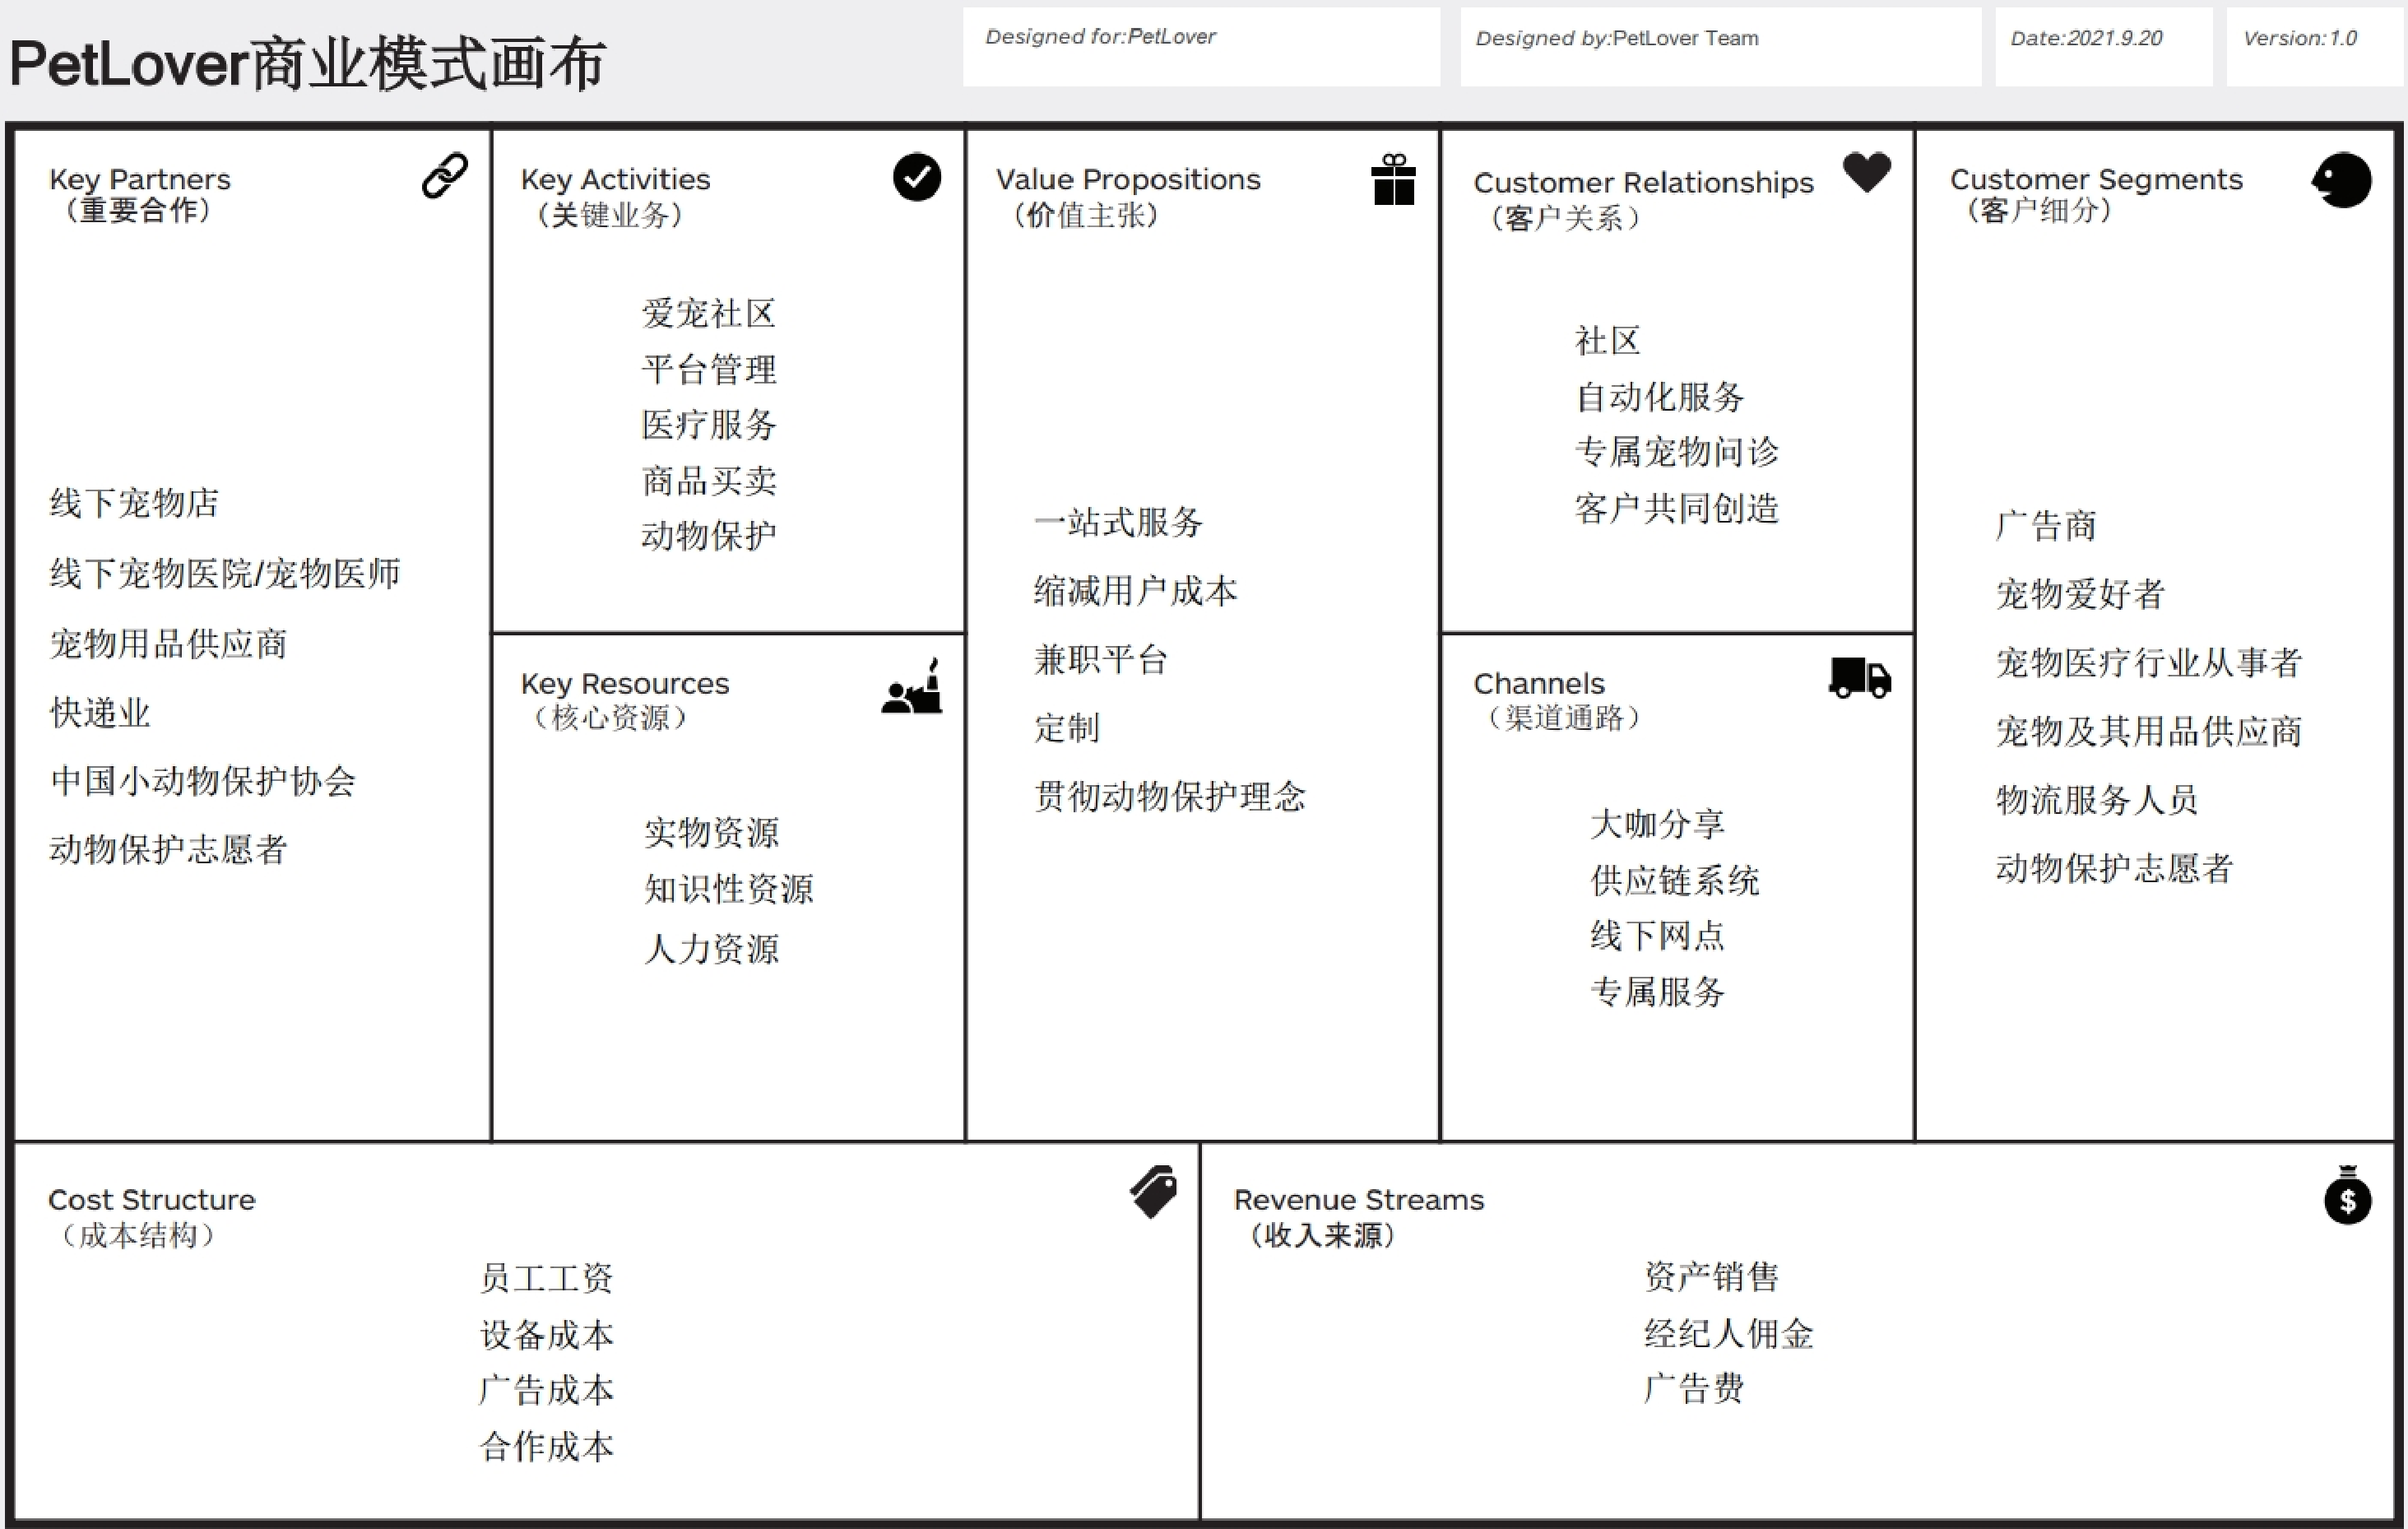
\includegraphics[width=16cm]{the-business-model-canvas}
\end{center}

\subsection{要点介绍}

\subsubsection{关键业务}

\begin{enumerate}[label=\alph*.]
  \item 添加业务。。。
\end{enumerate}

\subsubsection{价值主张}

\begin{enumerate}[label=\alph*.]
  \item 添加价值主张。。。
\end{enumerate}

\subsubsection{客户细分}

\begin{enumerate}[label=\alph*.]
  \item 添加客户细分。。。
\end{enumerate}

\subsubsection{客户关系}

\begin{enumerate}[label=\alph*.]
  \item 添加客户关系。。。
\end{enumerate}

\subsubsection{核心资源}

\begin{enumerate}[label=\alph*.]
  \item 添加核心资源。。。
\end{enumerate}

\subsubsection{重要合作}

\begin{enumerate}[label=\alph*.]
  \item 添加重要合作。。。
\end{enumerate}

\subsubsection{成本结构}

\begin{enumerate}[label=\alph*.]
  \item 成本结构
\end{enumerate}

\subsubsection{收入来源}

\begin{enumerate}[label=\alph*.]
  \item 添加收入来源。。。
\end{enumerate}

\subsubsection{渠道通路}

\begin{enumerate}[label=\alph*.]
  \item 添加渠道通路
\end{enumerate}


\subsection{要点联系}

\paragraph{1a(也就是关键业务的第一项), 2a(也就是价值主张的第一项)}阐述二者关系
\paragraph{。。。}阐述二者关系
\end{document}